\section{Special-Use IPv4 Addresses ; \texttt{rfc3300}}
\subsection{Private Network Addresses}
3 Address spaces are mentioned as ones
dedicated to private networks are mentioned
in the document:
\begin{enumerate}
	\item \texttt{10.0.0.0/8}\\
		A private network using this adress space might have up to $2^{32-8}$ devices.
	\item \texttt{172.16.0/12} -
		Max devices: $2^{32-12}$.
	\item \texttt{192.88.0/16}
		Max devices: $2^{32-16}$.
\end{enumerate}

\subsection{Contemporary usage of private network address spaces}

The private networks are now mainly used for increasing the amount
of devices that could be put in a single adress space
- by using the private address spaces in conjunction with NAT;
This enables the use of a single IPv4 address for many devices
which are all in the 'private network' of the gateway.\\

On the one hand - this solution makes networks that use it
much more compilcated and confusing to configure.\\
On the other hand this likely decreases the amount 
of public IPv4 addresses in use by an order of magnitude,
which not only helps us keep using IPv4 with more devices than there are
adresses - but more importantly helps keep routing tables smaller.

\section{Subnet Addressing in IPv4}
\subsection{}
\begin{enumerate}[label=\alph*.]
	\item The maximum amount of hosts is $2^{32-20}$
	\item In the Original Classful schemes,
		all addresses that start with a value between 128 and 191\footnote{Corresponding to \texttt{10******}},
		are class B addresses - including this one.
\end{enumerate}
\subsection{}
The address \texttt{78.12.100.0/21} only has only 11 bits
allocated to host suffix, so addresses inside it must match it in the first 21 bits.\\
In binary form:
\begin{verbatim}
_. 01001110.00001100.01100100.00000000 (78.12.100.0)
----------------------><-----------
a. 01001110.00001100.01100100.00001110 (78.12.100.14)
b. 01001110.00010101.01100100.00000001 (78.21.100.1)
c. 01001110.00001100.00000000.00000001 (78.12.0.1)
d. 01001110.00001100.01100000.00000000 (78.12.96.0)
e. 01001110.00001100.01101100.00000000 (78.12.108.0)
\end{verbatim}
After looking carefully, we see that only a,d and e match in the first 21 bits.
\begin{enumerate}[label=\alph*.]
	\item \texttt{78.12.100.14} -  in network.
	\item \texttt{78.21.100.1} - not in network.
	\item \texttt{78.12.0.1} - not in network.
	\item \texttt{78.12.96.0} - in network.
	\item \texttt{78.12.108.0} - in network.
\end{enumerate}

\subsection{}
\begin{enumerate}[label=\alph*.]
	\item The subnet mask: \texttt{255.255.192.0}. The network addresses:
	\begin{itemize}
		\item \texttt{130.62.0.0/18}
		\item \texttt{130.62.64.0/18}
		\item \texttt{130.62.128.0/18}
		\item \texttt{130.62.192.0/18}
	\end{itemize}
	\item The subnet mask: \texttt{255.255.252.0}. The network addresses:
	\begin{itemize}
		\item \texttt{130.62.0.0/22}
		\item \texttt{130.62.4.0/22}
	\end{itemize}
	\item The subnet mask: \texttt{255.255.252.0}. The network addresses:
	\begin{itemize}
		\item \texttt{130.62.0.0/18}
		\item \texttt{130.62.4.0/18}
		\item \texttt{130.62.8.0/18}
		\item ...
		\item \texttt{130.62.252.0/18}
	\end{itemize}
\end{enumerate}

\section{Routing Configuration Utilities Overview}
\subsection{ARP cache}
\begin{enumerate}[label=\alph*.]
	\item
	My connection interface is:
	\begin{verbatim}
		Wireless LAN adapter Wi-Fi:
	
	   Connection-specific DNS Suffix  . : technion.ac.il
	   IPv4 Address. . . . . . . . . . . : 192.168.59.127
	   Subnet Mask . . . . . . . . . . . : 255.255.252.0
	   Default Gateway . . . . . . . . . : 192.168.56.1
	\end{verbatim}
	
	And the ARP cache contains:
	\begin{verbatim}
		C:\Users\pc>arp -a 192.168.56.1
	
		Interface: 192.168.59.127 --- 0x7
		Internet Address      Physical Address      Type
		192.168.56.1          00-09-0f-09-00-06     dynamic
	\end{verbatim}
	so \texttt{00-09-0f-09-00-06} is the MAC address of my default gateway.
	
	\item All of the relevant packets have been highlighted.\\
	The first two highlighted packets are from the ARP protocol.\\
	The rest of the highlighted packets are for the ICMP protocol itself.
	\begin{center}
		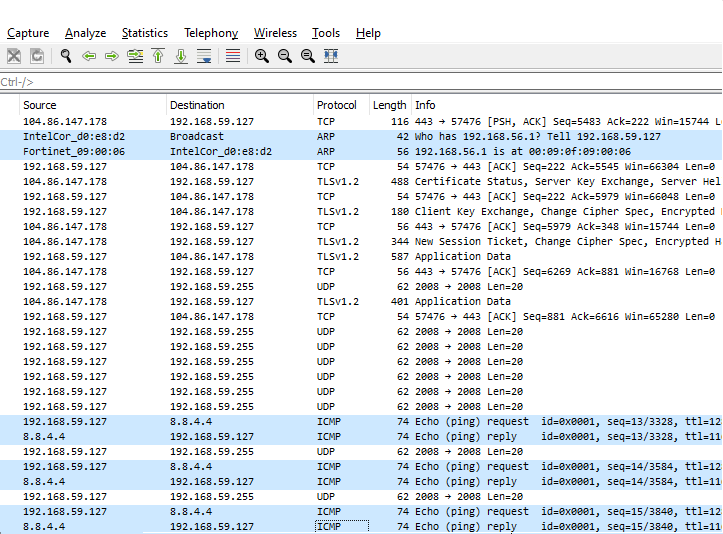
\includegraphics[width=1.2 \textwidth]{Resources/del_arp_cache.png}\centering
	\end{center}
	\begin{itemize}
		\item The purpose of the first packet isto find out what is the physical (MAC) address
		of the default gateway. This is required since at that point - the 
		arp cache at the gateway's entry was empty since we have just deleted it.
		\item The second packet is a response to the first one (Still ARP protocol), and it 
		specifies the value of the requested address.\\
		Without this preceeding ARP interaction - the host would not know
		how to interact with the default gateway.
		\item The next 6 packets are a part of the ICMP protocol. The 
		first one requests a response from the host at \texttt{8.8.4.4},
		and the next packet is the response from \texttt{8.8.4.4} back to the requester.\\
		The third packet is also a request for response and the next on is the response, and so on.
	\end{itemize}
	\item If we were to run the \texttt{ping 8.8.4.4} command again - 
	we would not see the same packets transfered - since there would be 
	no need for the ARP packets this time, the IP to MAC address mapping
	for the default gateway is already cached and there is no need to querry for it again.
	\item Sending \texttt{ping 8.8.4.4–l 4000} results with:
	\begin{center}
		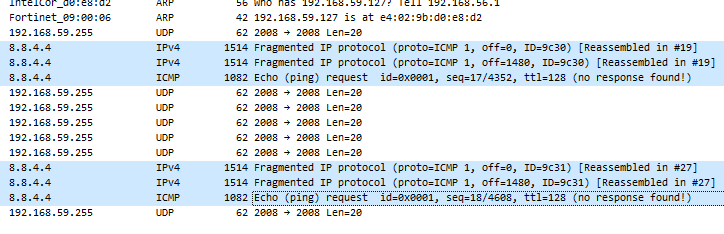
\includegraphics[width=1.2 \textwidth]{Resources/icmp_frag.png}
	\end{center} 
	\begin{enumerate}
		\item Each ICMP request was split into three fragments,
		This is since the MTU for the system is 1500 bytes, meaning 
		at-least 3 fragmets are required to contain a 4000-byte
		message.
		\item IPv4 Header details:
		\begin{center}
			\begin{tabular}{ |c|c|c|c|c|c| } 
			\hline
			Checksum & Fragment Offset & Flags & Id & Total Length & \#Fragments \\ 
			\hline
			0x70bd   & 0 			   & 001   & 0x9c30  & 1500	   & 1			 \\ 
			0x7004   & 1480 		   & 001   & 0x9c30  & 1500	   & 2			 \\ 
			0x90fb   & 2960 		   & 000   & 0x9c30  & 1068	   & 3			 \\ 
			\hline
			\end{tabular}
		\end{center}
		\item A service that supports fragmeted ICMP exposes itself to DOS attacks.\\
		This is since fragmeted packets require the reciver to save a state (and allocate resources)
		for each sender; moreover - unlike a regular http session - ICMP is not built on TCP,
		and so no 3 way TCP handshake was used to authenticate the sender IP address - which means
		IP spoofing can be used in a potential DOS attack.
		\item \begin{verbatim}
			C:\WINDOWS\system32>ping localhost -l 4000

			Pinging DESKTOP-86KTLQ1 [::1] with 4000 bytes of data:
			Reply from ::1: time<1ms
			Reply from ::1: time<1ms
			Reply from ::1: time<1ms
			Reply from ::1: time<1ms

			Ping statistics for ::1:
				Packets: Sent = 4, Received = 4, Lost = 0 (0% loss),
			Approximate round trip times in milli-seconds:
				Minimum = 0ms, Maximum = 0ms, Average = 0ms
		\end{verbatim}
	\end{enumerate}
\end{enumerate}

\subsection{\texttt{tracert}}
\begin{enumerate}[label=\alph*.]
	\item The type field value is 8, which means it's a ping request.
	\item The responses have type 11, which means the request packet has
	exceeded it's time-to-live value.
	\item \texttt{tracert} works as follows:
	\begin{enumerate}[label=\arabic*.]
		\item \texttt{tracert} sends a series of ICMP packets, each
		 with an increasing \texttt{TTL} (Time To Live) value, starting from 1.
		\item The first packet with \texttt{TTL=1} is sent to the target IP address.
		 When the packet reaches the first router (the router closest to my computer), the \texttt{TTL} value is decremented by 1,
		 and the router sends an \texttt{ICMP Time Exceeded} message back to my computer.\\
		 Traceroute might also repeat each step multiple times to verify that the routing through a specific
		 node is consistent; in the case of our experiment - it repeats each step 3 times.
		\begin{figure}
			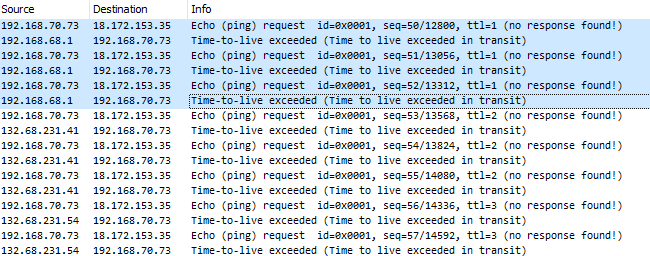
\includegraphics[width=1.2 \textwidth]{Resources/tracert_ws.png}
			\caption{The first 6 packets seen have identified the first router in the path to \texttt{www.walla.co.il},
			each pair is a ping request, followed by a response from the router at the distance that equals to the value of the \texttt{TTL} (which is 1),
			and the interaction is repeated 3 times. The following 6 packets are used to identify the next router in the path - at the distance of 2, and so on.}
		\end{figure}
		\item The \texttt{tracert} command records the IP address of the router
		 that sent the Time Exceeded message, along with the round-trip time it took for the packet to travel to and from that router.
		\item The \texttt{tracert} command then sends another ICMP packet with a
		\texttt{TTL} value of 2. This packet will reach the first router and be forwarded to the next router along the path to the target IP address.
		\item The process repeats, with the \texttt{TTL} value increasing by 1 each
		 time until the target IP address is reached or a maximum number of hops is reached.
	\end{enumerate}
	\item There are a few reasons why this method of detecting the routing path might yield
	false results: firstly - the routing path might change between packet to packet
	depending on how routers on the way might decide the optimal routing is at that moment.
	Moreover - some routers on the way might not respond to the timed-out ICMP packets the way we expect.
	For example - some might give a replay after dropping a timed-out packet.
\end{enumerate}

\section{DHCP ; \texttt{RFC 2131}}
\subsection{Wireshark Analysis}
\begin{figure}
	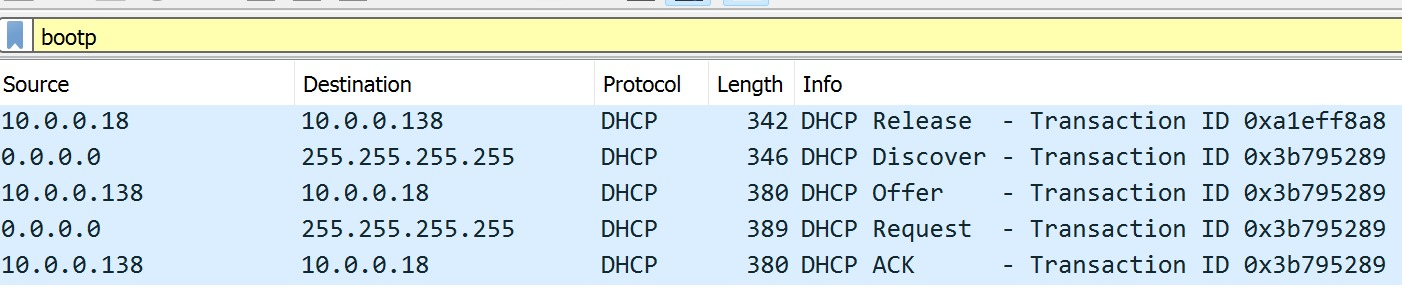
\includegraphics[width=1.2 \textwidth]{Resources/dhcp_ws.jpeg}
	\caption{The DHCP messages include the first one from previously releasing
	the allocated address, followed by Discover, Offer, Request and ACK messages.}
\end{figure}
The DHCP server needs to know the MAC address since it's
the only way it can identify the client (if it already had an IP
it would not need DHCP!), moreover - just because the
MAC address appears in the packet does not mean it gets to the DHCP server
as layer 2 headers (including the MAC address) are not passed on to
the protocols above them.

\subsection{}
It is the same address. This means that the client and server 
are directly connected at layer 2,
and that no DHCP relay is required for the two to communicate.
\begin{figure}
	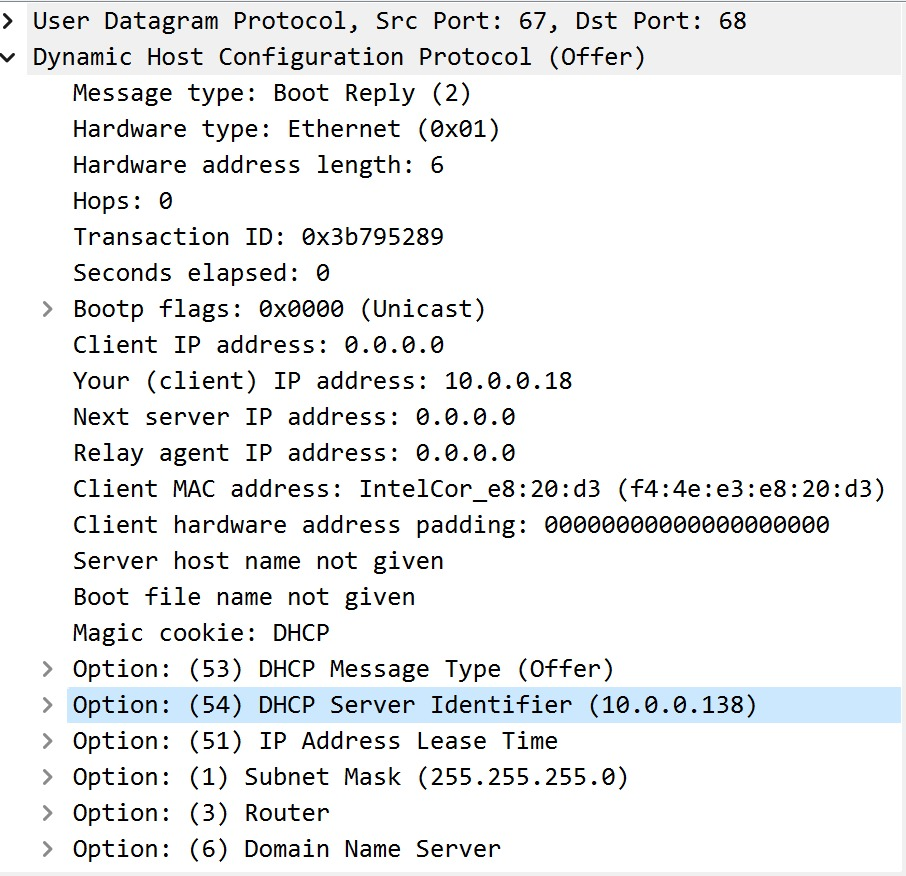
\includegraphics[width=1.2 \textwidth]{Resources/dhcp_srv.jpeg}
	\caption{As can be seen, the DHCP server address is the same address
	that is sending the DHCP server messages back to the client.}
\end{figure}

\subsection{}
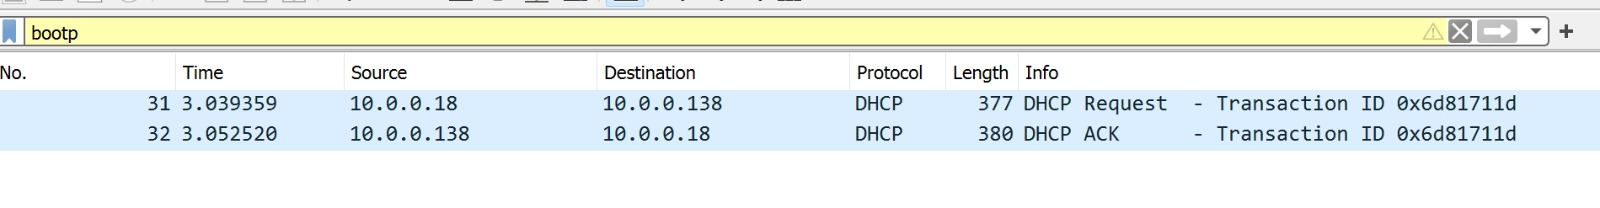
\includegraphics[width=1.2\textwidth]{Resources/dhcp_renew.jpeg}
No new DHCP messages were sent during the 10 minutes.\\
This means that the lease time is more than 20 minutes - since 
after half the lease time has expired - the client is meant to send 
a DHCP Request message to renew it's lease.\\
The lease time is dictated by the DHCP server,
it's timing can be controled by it's configuration, or the lease
time requested.\\
When deciding what the lease time should be - there is a trade-off:
have a lease time which is too long might mean a-lot 
of unused addresses are still allocated to hosts which
did not relase them properly when they where done using them,
and on the other hand - having too short
of a lease time will cause unnssecery traffic that might
take bandwidth that could otherwise be used for something else.

\subsection{}
\begin{enumerate}[label=\alph*.]
	\item In it's DHCP request, the server will use
	option number 61, type 1; and provide \texttt{192.168.32.32}
	as it's requested address.
	\item The server will specify options 3, 6 and 1 in it's request.
	\item The server should specify option 51,
	and provide the lease time value in seconds (so the number of seconds in a week).
\end{enumerate}

\section{OSPF ; \texttt{RFC 2328}}
\subsection{}
In the context of the Directed Graph data scructure saved for the OSPF
protocol, each node represents a router or a whole Local-Area-Network, while an arch represents
a physical-layer-connection between two nodes s.t. information will be forwarded in the direction of the arch.\\
For example router-router connection
means that the two routers will forward information to eachother (depending on the arch direction) at layer 2, and a router to LAN connection
means that the router will forward information to the LAN.

\subsection{}
Since a stub network is only connected to that one router - there is
no possiblity that the stub network will every forward any information from
a different network through itself and into it's gateway router.

\subsection{}
The main difference between Brodcast networks and NBMA networks
is that the latter do not support brodcasting messages.\\
This also means that if node $A$ in the DHCP graph is from outside an
NBMA network with multiple is connected to node $B$ inside
tehe NBMA network - it might still not be able to directly communicate
with another router $C$ which is also inside the same NBMA network;
this means that the router $B$ will likely be required to forward information between
routers $A$ and $C$ - and hence the connection to it should be bi-directional.

\subsection{}
A 'point-to-point' connection is a direct connection between
two routers - by a single packet transfer on the underlying layer
2 protocol.\\
Such a connection will be saved as a 'type 1' (point-to-point) link descriptor,
with link ID equal to the IP of the neighboring router.\\
Additionally - such a connection will create another 'type 3' link desciptor,
which represents a stub link, similarly with the router's IP
as the ID.

\subsection{}
Large AS's are often divided into distinct regions,
and the routers in each region are only required to hold
the relavant data structures to the routers in their own regions.\\
When inter-regional routing is needed - the routing is done through what's
called the 'backbone' of the OSPF network; this backbone is
one of the regions that comprize the AS and it essentially
acts as a hub for the AS through which the inter-regional
communications is transmitted.

\subsection{}
The five message types that exist in OSPF are:
\begin{enumerate}
	\item Hello: These messages are essentially ping messages
	used to discover and maintain who the router's neighbors are.
	\item Database Description: These messages summerize
	the content of the database saved in the sending router,
	which enables others to update their own database accordingly.
	\item Link State Request: These messages are requests to
	recive other's databases.
	\item Link State Update: These messages request other's
	to update their own databases.
	\item Link State Ack: These message indicate that a required database
	update has been completed. The use of these acknolagments helps
	improve the reliability of the protocol in cases of unreliable connections
	or crashes.
\end{enumerate}
